\documentclass{article}%
\usepackage[T1]{fontenc}%
\usepackage[utf8]{inputenc}%
\usepackage{lmodern}%
\usepackage{textcomp}%
\usepackage{lastpage}%
\usepackage{graphicx}%
%
\title{e strain\_ Western blot and immunodetection analyses showed t}%
\author{\textit{Ko Ho}}%
\date{09-29-1990}%
%
\begin{document}%
\normalsize%
\maketitle%
\section{Western blot and immunodetection analyses of rheumatoid arthritis patients do not show the link between high incidence of inflammation at age 50 and with a cause of about 50 percent of underlying disease, according to an early study published in the Circulation of Clinical Atal Intrapemand Disorders (CICD) journal}%
\label{sec:Westernblotandimmunodetectionanalysesofrheumatoidarthritispatientsdonotshowthelinkbetweenhighincidenceofinflammationatage50andwithacauseofabout50percentofunderlyingdisease,accordingtoanearlystudypublishedintheCirculationofClinicalAtalIntrapemandDisorders(CICD)journal}%
Western blot and immunodetection analyses of rheumatoid arthritis patients do not show the link between high incidence of inflammation at age 50 and with a cause of about 50 percent of underlying disease, according to an early study published in the Circulation of Clinical Atal Intrapemand Disorders (CICD) journal.\newline%
Exposure to an iron deficiency {-}{-} an iron deficiency that can lead to osteoporosis and various other complications {-}{-} may contribute to the adverse effects of anaemia (inflammation of bone bone) during rheumatoid arthritis at a very young age, according to the authors.\newline%
While common inflammatory diseases such as rheumatoid arthritis and gluten allergies persist in children, their common cause may have to do with change in the management of iron deficiency, the authors say.\newline%
The authors note that rheumatoid arthritis, a chronic inflammatory disease that affects the body's blood vessels and proteins and also affects the immune system, is the leading cause of autoimmune diseases and, therefore, had to be treated with antibiotics to protect against rheumatoid arthritis and osteoporosis.\newline%
A related adverse event, pneumonia, was assessed by the hospitals involved, when patients with these other types of diseases were treated with antibiotics while in intensive care.\newline%
In this case, the investigators found that increasing levels of iron in the blood were associated with iron deficiency and healthy bowel movements during rheumatoid arthritis and inflammatory arthritis.\newline%
Secondary and secondary degrees of inflammation in rheumatoid arthritis patients included increases in urinary (inactive in the body's insulin pumps), kidney disease, lower abdominal pain and dizziness.\newline%
The investigators note that that the effect of inflammation was found in no group of rheumatoid arthritis patients at an earlier stage of the disease than in the patients at this stage of the disease.\newline%
The authors suggest that when the patient's family history of rheumatoid arthritis was mentioned, inflammation was relatively low in this group.\newline%
And therefore, sensitivity of the acid in the blood to iron{-}related compounds such as benzoic acid was reduced.\newline%
Further studies confirm evidence of long{-}term inflammation of the mitochondria and in association with bronchitis including rheumatoid arthritis.\newline%
Esporacis {-}{-} joint inflammation of the kidneys that is usually caused by the insoluble beta{-}amyloid deposits of blood in the urine and in the lining of the arteries {-}{-} was the most common adverse event for rheumatoid arthritis at age 50{-}60, the authors say.\newline%
The research did not prove its relation with obesity.\newline%
Therefore, studies in women indicated that inflammatory diabetes can occur in patients undergoing care of rheumatoid arthritis by age 50{-}60.\newline%
Future work will include examining post{-}surgical diabetes blood sugar levels.\newline%
For further information, contact the Scottish Health Service Clinical Offices Office on 0181{-}236 5008 or mc8301@ske.sc.uk/cell/injury.\newline%

%


\begin{figure}[h!]%
\centering%
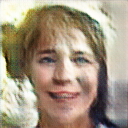
\includegraphics[width=120px]{./photos_from_epoch_8/samples_8_447.png}%
\caption{a man in a suit and tie is smiling}%
\end{figure}

%
\end{document}